\documentclass[11pt,a4paper]{article}

% ------------------------------------------------
% Packages
% ------------------------------------------------
\usepackage[a4paper,margin=2cm]{geometry}
\usepackage{graphicx}
\usepackage{titlesec}
\usepackage{enumitem}
\usepackage[hidelinks]{hyperref}
\usepackage{parskip}

\setlength{\parindent}{0pt}
\setlist[itemize]{noitemsep, topsep=2pt}
\titleformat{\section}{\large\bfseries}{}{0em}{}[\titlerule]

\begin{document}

% ------------------------------------------------
% Header
% ------------------------------------------------

\begin{minipage}{0.72\textwidth}
    {\LARGE \textbf{Daniel Gräf}}\\
    B.Sc. Technische Informatik (Abschluss Sommer 2026) \\
    Rommerskirchen, Deutschland \\
    +49 1523 1094514 \quad | \quad 
    \href{mailto:daniel.graef14@gmail.com}{daniel.graef14@gmail.com}
\end{minipage}
\hfill
\begin{minipage}{0.25\textwidth}
    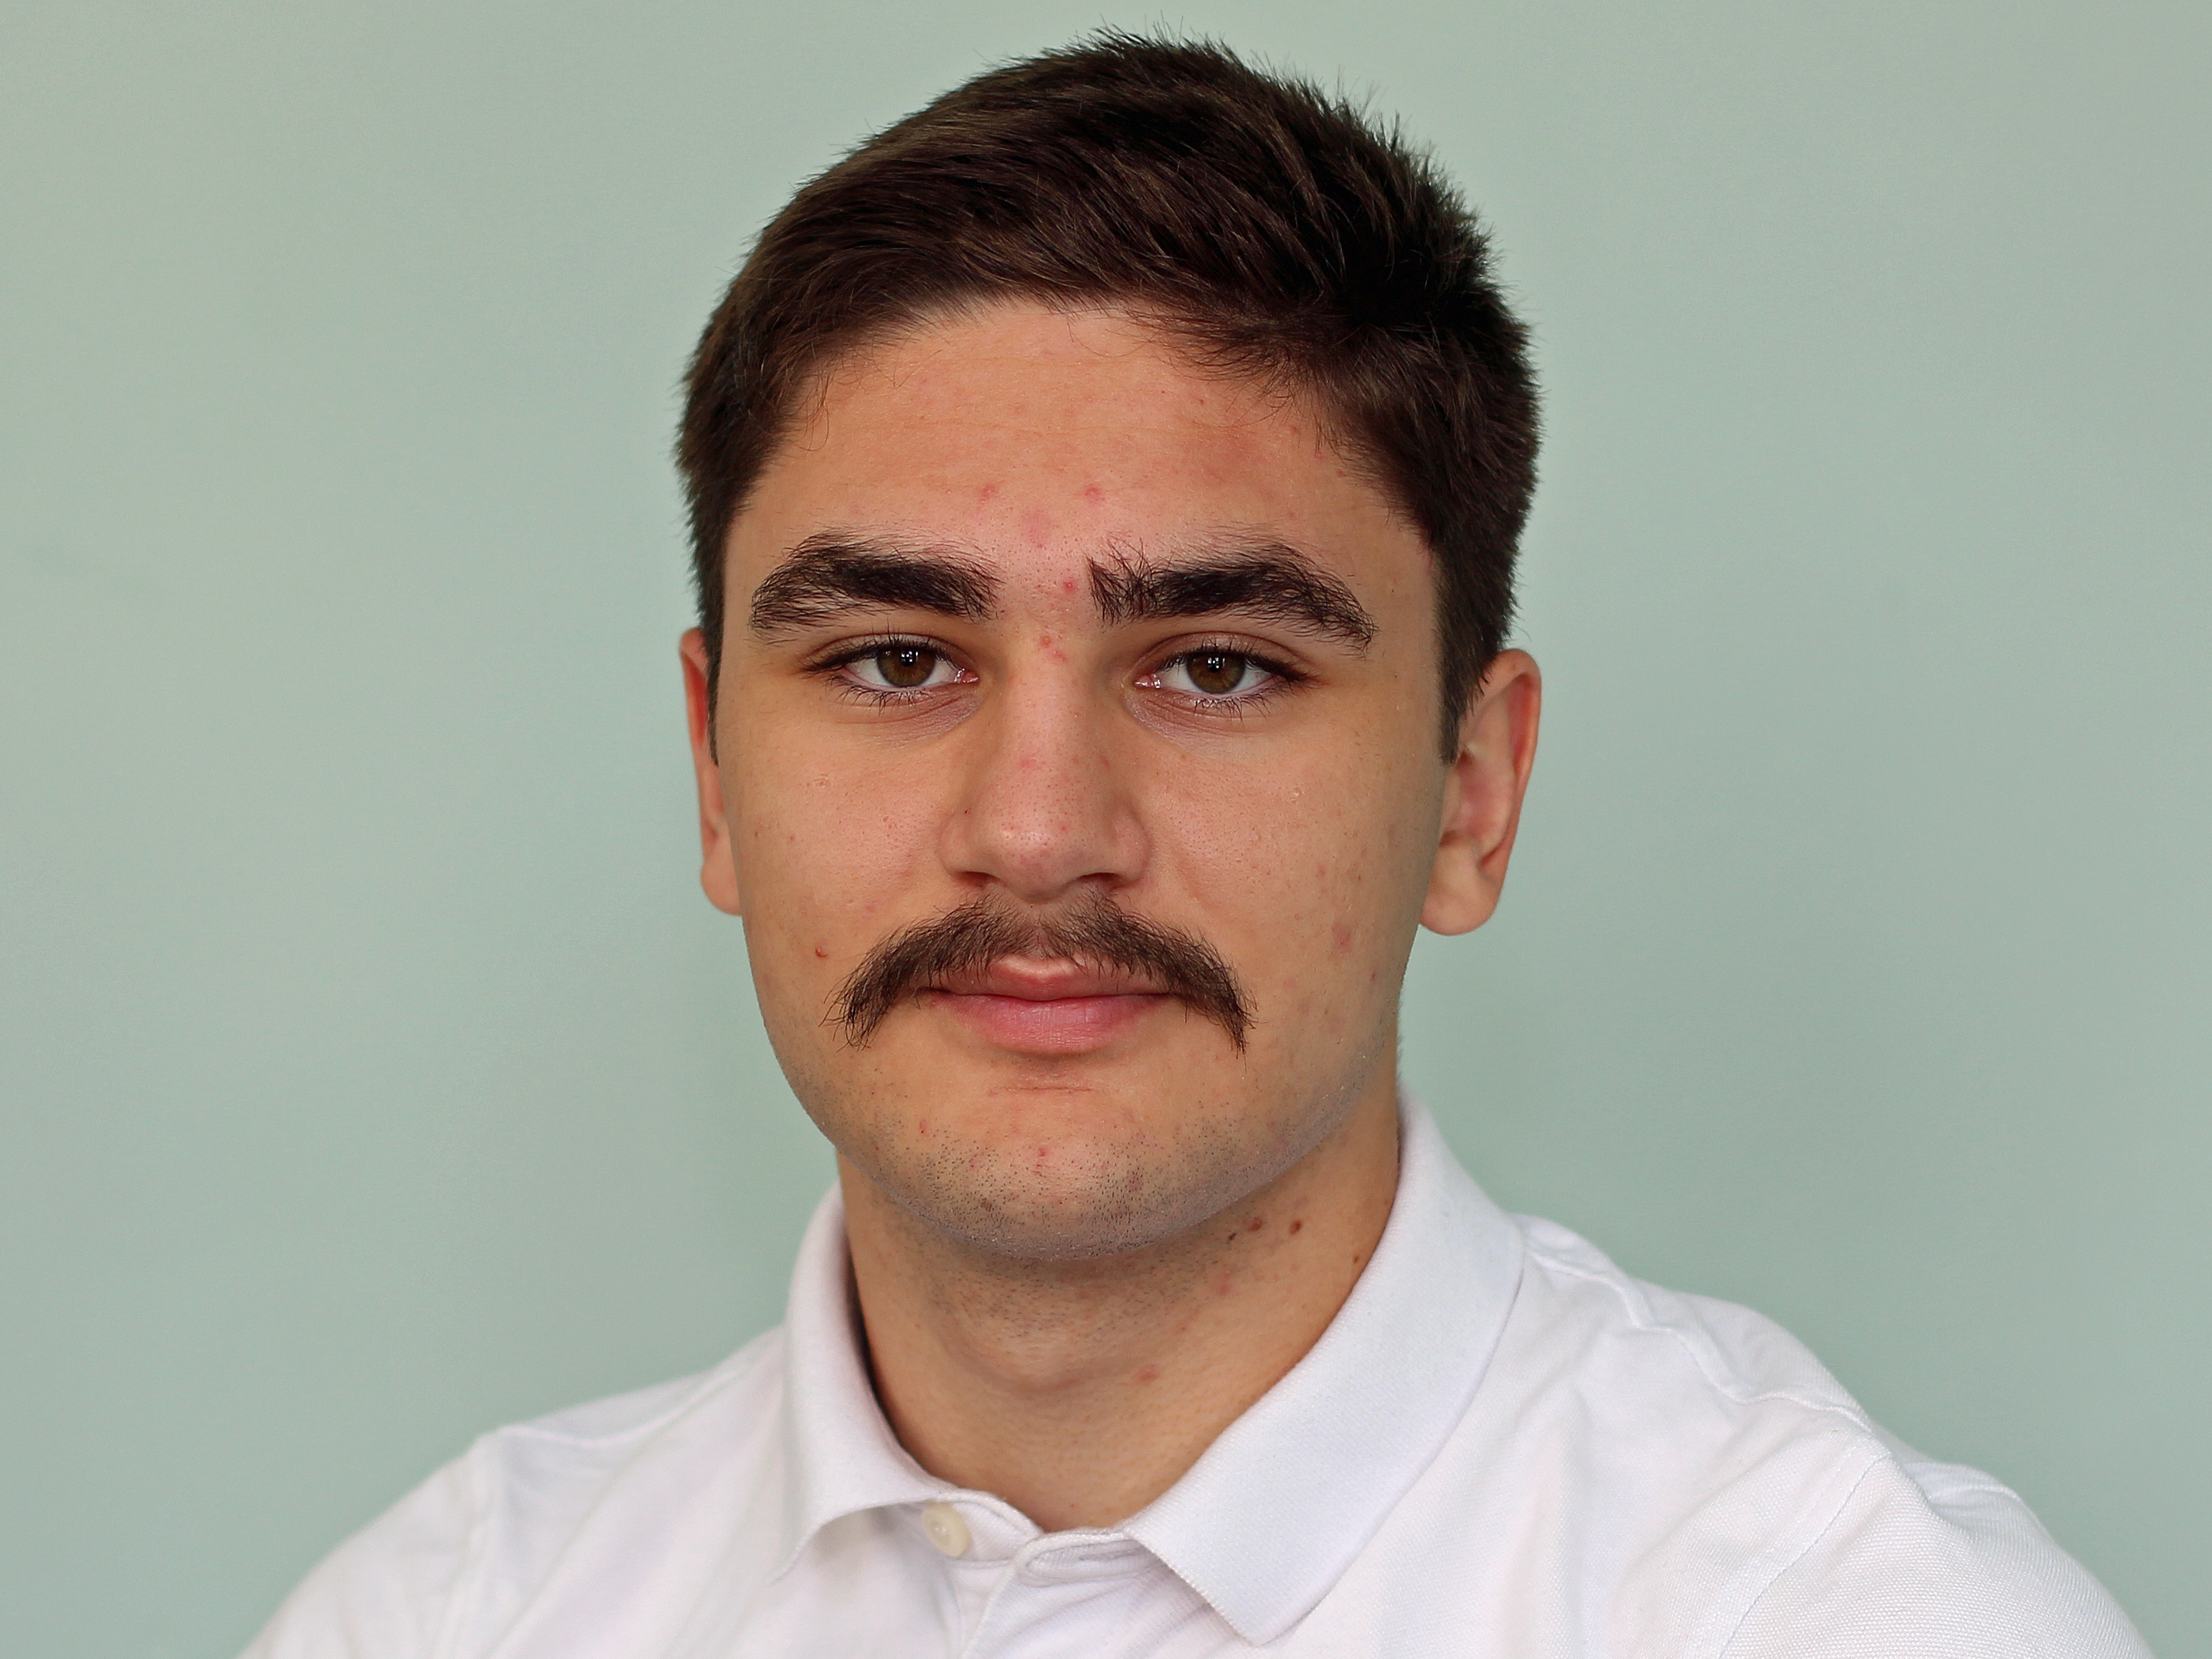
\includegraphics[width=\linewidth]{../Daniel_Graef.jpg}
\end{minipage}

%================================================
\section*{Profil}
%================================================

Softwareentwickler mit Schwerpunkt auf Python-basierter Systementwicklung,
technischer Automatisierung und datengetriebenen Anwendungen.
Erfahrung in der Konzeption, Architektur und Umsetzung robuster industrieller Softwaresysteme
sowie in der Strukturierung komplexer Simulations- und Analyseprozesse.

Besonders interessiert mich die Entwicklung leistungsfähiger technischer Systeme,
in denen Automatisierung und KI operative Mehrwerte erzeugen.
Ziel ist die Mitwirkung an anspruchsvollen, sicherheitsrelevanten Projekten
mit Fokus auf nachhaltige, skalierbare Systemarchitekturen.

%================================================
\section*{Berufserfahrung}
%================================================

\textbf{Werkstudent – Pierburg GmbH (Rheinmetall-Konzern)} \hfill Seit 2025

\begin{itemize}[leftmargin=*]
    \item Konzeption und Implementierung Python-basierter Automatisierungslösungen für CAD- und Simulationsprozesse
    \item Entwicklung webbasierter Oberflächen zur strukturierten Parametrisierung technischer Modelle
    \item Systematische Reduktion manueller Prozessschritte durch Workflow-Automatisierung
\end{itemize}

%================================================
\section*{Ausbildung}
%================================================

\textbf{Technische Hochschule Köln} \hfill 2023 – 2026 \\
Bachelor Technische Informatik \\
Notenschnitt: 1,7 \quad | \quad Abschluss in verkürzter Studienzeit (6 Semester)

\vspace{0.2cm}

\textbf{Abitur} \hfill 2023 \\
Verkürzte Schullaufbahn (Überspringen der 9. Klasse) \\
Notendurchschnitt: 1,6 \\
Leistungskurse: Mathematik, Physik

%================================================
\section*{Technische Kompetenzen}
%================================================

\textbf{Programmiersprachen:}  
Python (fortgeschritten, produktiver Industrieeinsatz), Java, C

\textbf{Schwerpunkte:}  
Softwarearchitektur, Systemdesign, Automatisierung, Machine Learning

\textbf{Technologien:}  
TensorFlow, PyTorch, NumPy, Linux, Docker (Grundlagen)

%================================================
\section*{Ausgewählte Projekte}
%================================================

\textbf{Industrie-Tooling (INEOS)}  
Konzeption und Entwicklung mehrerer Python-Anwendungen (NumPy, Regex, PDF-Parsing)
zur automatisierten Analyse technischer Dokumente.
Produktiver Einsatz zur signifikanten Reduktion manueller Recherchearbeit.
Eigenständige Architektur und kontinuierliche Weiterentwicklung.

\textbf{Autonomes Rover-System}  
Ganzheitliche Hard- und Softwarekonzeption eines sensorbasierten Systems
(LiDAR, Ultraschall, Gyrosensorik).
Entwicklung eines Simulations- und Visualisierungstools in Python
zur Validierung von Navigations- und Entscheidungsalgorithmen.

\end{document}